\chapter{Overview of techniques}
This chapter introduces the techniques used to simulate destructible environments. First, we talk about the development of the destructible environment in several games and game engines, then about general approaches to this problem.

We will repeatedly categorise the content of the game world in following way: We will use the word \emph{object} to refer to any building, crate, door, tree or other items that occur in the game environment, but excluding terrain, distant environment like skyboxes and any in-game characters. Most of the modern 3D games use the term destructible environment as a reference to destructible objects because they do not support the destruction of terrain. We will comply with this terminology and, unless specified otherwise, use the term destructible environment as a reference to a destruction of game objects and not the terrain.

\section{Implementations in mainstream gaming}
\label{sec:common}
In this brief overview, we introduce the most common approaches to environment destruction that can be seen through the games released in last 40 years. More common approaches can be seen used in newly released games.

\para{Object replacement or removal} was the first~\cite{history} method used to simulate a destructible environment in a computer game, mostly because it is straightforward and undemanding. This approach is based on swapping models or any other kind of visual representations, for more damaged ones or completely removing them. Because it relies on pre-made models, exact collision points on the models are not considered, and the result is always the same. If we were to consider $N$ points of taking damage, the number of different models could grow up to $2^N$. A large number of models is not practical for game development, other approaches are therefore used for breaking the object at the precise point. Despite its simplicity and limitations, this approach can still produce a very desirable result. In fact, it is still most widely used approach to a destructible environment in computer games.

In our simplified view on 2D games, we will not differentiate between objects and terrain and refer to both as the environment.
First 2D games featuring the destructible environment were arcade games like the \emph{Space Invaders (1978)}\footnote{\url{https://en.wikipedia.org/wiki/Space\_Invaders}} where the environment is represented by cells in a grid. After taking damage, the visual representation of the cell is replaced by one looking more damaged and the finally completely removed. About a decade later, new environment destruction technique was used in games like \emph{Scorched Earth (1991)}\footnote{\url{https://en.wikipedia.org/wiki/Scorched\_Earth\_(video\_game)}} and \emph{Worms (1995)}\footnote{\url{https://www.team17.com/games/worms-original}}. Collision and removal of terrain in those games is based on individual pixels rather than whole objects, which creates a more realistic visual effect. In \emph{Scorched earth} players typically need to blow away a hill dividing them, in \emph{Worms} it is common to dig a tunnel to hide from your enemies gunfire.

In 3D games, the principal technique of implementation of destructible objects has not changed much over the years. For every object that the player can modify there is a prepared set of alternative models with various amount of damage applied. Based on how much damage is applied, the models are swapped and eventually completely removed, as seen in \cref{fig:doors}. Swapping the models is usually accompanied by animations, debris and dust generation, designed to hide the unrealistically instant change of the object from the player. The disadvantage of this method is the necessity to replace the in-game objects as a whole --- there has to be a significant number of objects pre-made for different scenarios to make the game look realistic. A small number of pre-made damaged models means this approach can not flexibly react to specific player actions. As an example, in the \emph{Source} engine, the hole in the door (\cref{fig:doors}) is always created at the same place, regardless of the point of the impact. Another example can be found in the game \emph{Duke Nukem 3D}\footnote{https://en.wikipedia.org/wiki/Duke\_Nukem\_3D}, where specific parts of the walls are created as separate objects that disappear when hit.

\begin{figure} 
\centering
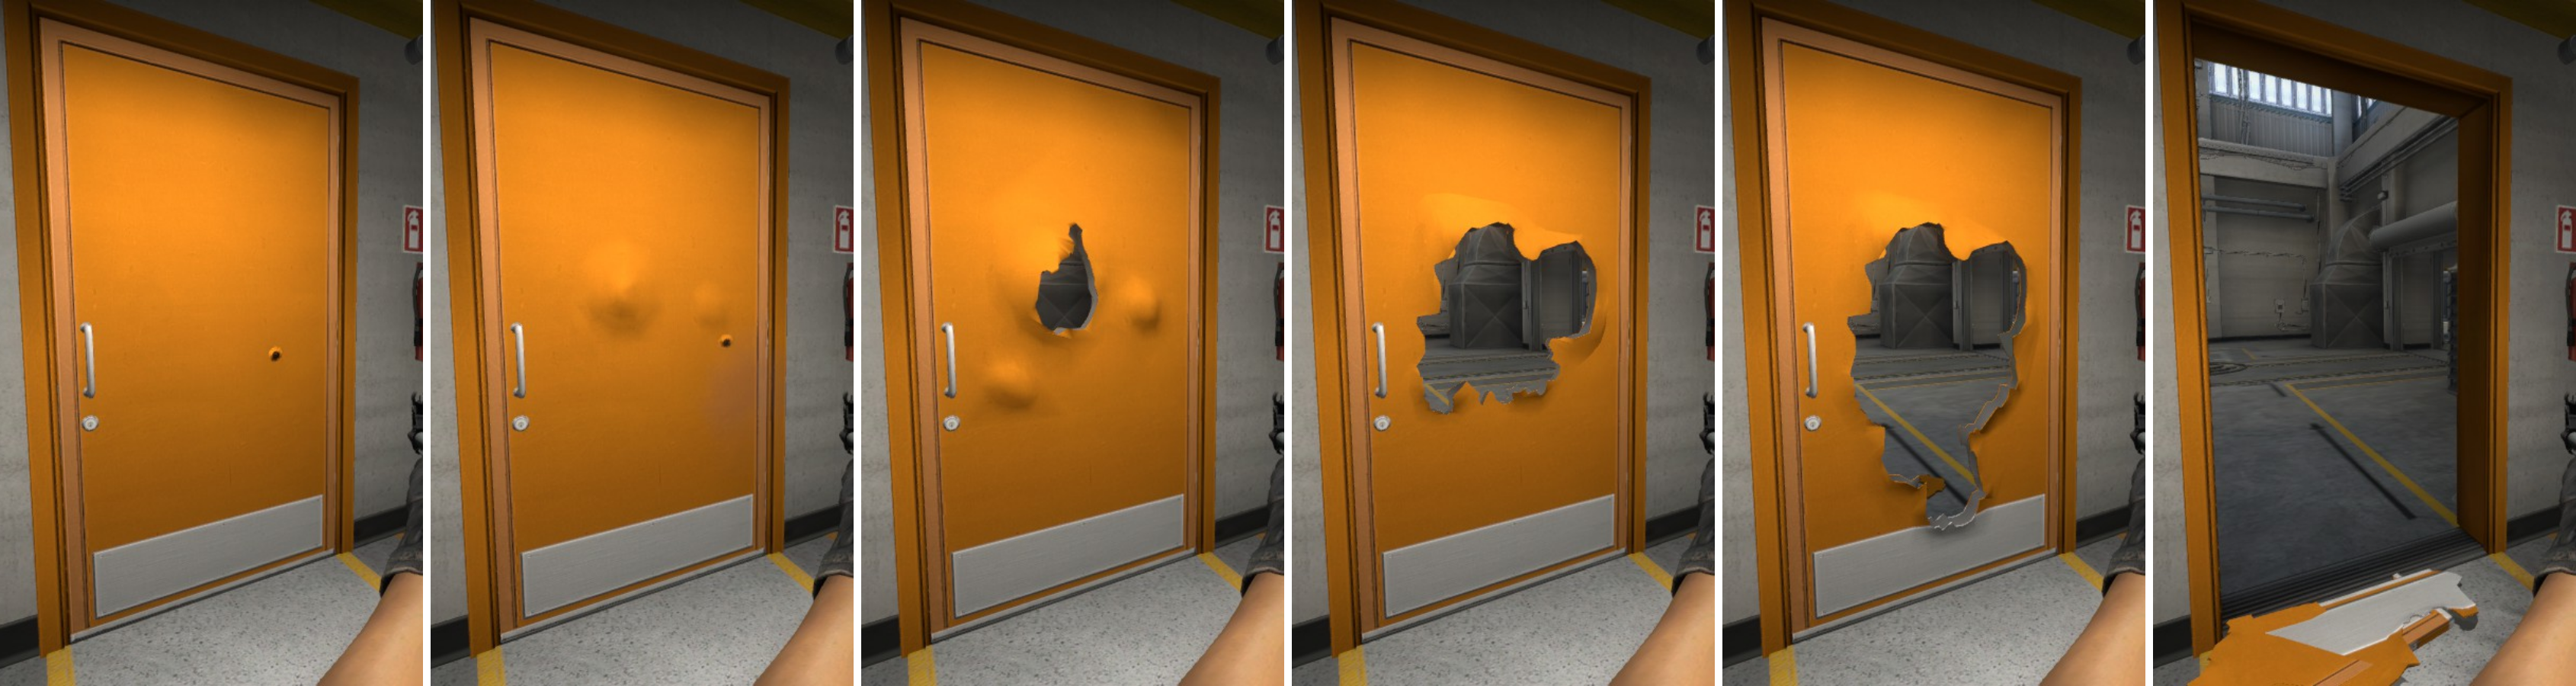
\includegraphics[width=\textwidth]{img/doors}
\caption{\emph{Source} engine swaps door models. Image taken from \emph{Counter Strike: Global Offensive}. Successively damaging any doors in the game will always produce this sequence of models, regardless of the exact point where the damage was applied.}
\label{fig:doors}
\end{figure}

\para{Height map approach} is closely intertwined with terrain generation. The basic principle behind modifying the environment with this method is changing the height of the terrain at given point. We can find this method used in the first 3D games that featured destructible terrain, \eg \emph{Magic Carpet (1994)}~\footnote{\url{https://ultimatehistoryvideogames.jimdo.com/magic-carpet}} or \emph{Starfighter 3000 (1994)}~\footnote{\url{https://en.wikipedia.org/wiki/Star\_Fighter\_(video\_game)}}.

The height map of a 3D terrain is defined as a uniform 2D grid of values representing height of their respective column in 3D space. A convenient approach is to use 2D grey-scale bitmap and represent the height as a colour distance from the white colour, black being the maximum. Because the grid only contains information about the discrete points, interpolation is used to create continuous terrain. We can also view this method as creating a function of two coordinates on the plane giving us the value on the vertical axis. The definition of function forbids more than one function value at each input point, therefore this method can not represent multiple layers of terrain. The relative simplicity of the approach is counterweighted by the fact that it can only change the height of the terrain and does not allow creating caves, tunnels or similar hollow features.

\para{\emph{Geo-Mod}} (\emph{Geometry Modification Technology}\cite{geomod}) is an engine developed for the \emph{Red Faction (2001)}\footnote{\url{http://redfaction.wikia.com/wiki/Red\_Faction}} video game. It approaches the modification of the terrain by creating objects representing a empty space. After every collision, a new object is created at the point of collision. This new object is then subtracted from the terrain creating the modified terrain with the newly created hole. The difference of the meshes is calculated in real time. Even though the engine does not work well with the buildings and other objects \todo{tusime proc? nie :'(}, it represented the first significant attempt to create the fully destructible 3D environment that would work under real-time constraints.

\para{\emph{Geo-Mod 2}}~\cite{geomod}\footnote{Geo-Mod 2.0 presentation video \url{https://www.youtube.com/watch?v=lICurOVsNv0}} does not feature destructible terrain, instead, it focuses on realistic destruction of buildings. A set of smaller objects is used to represent each building as a ragdoll (multiple objects connected with joints) for the simulation of inner stresses. Switching from using a conventional 3D model to the ragdoll simulations, requires at least basic knowledge of civil engineering in order to properly analyse structural stability of the building and create a ragdoll model simulating it properly. This process is done by hand in the development process and can not be modified at a runtime. The high complexity of simulation limits the engine in the scale of the game world and mutual proximity of destructible objects. Because of that, game avoids any interaction of multiple buildings requiring simulating their behaviour at once.


\para{\emph{Frostbite}}~\footnote{http://www.frostbite.com/about/frostbite-3} engine (and mainly its component \emph{Destruction}~\cite{destruction}) is currently used in new mainstream games that feature destructible environment \eg \emph{Battlefield} series or \emph{Star Wars Battlefront (2015)}. It supports two different kinds of destruction micro-destruction on the surface and the large scale predetermined destruction on whole buildings. 

The dynamic micro-destruction focuses on creating small dents into the surface of the object. The dents are created dynamically at the point of impact and can be placed on any point of the surface.

The large-scale destruction is focused on destroying entire buildings. The buildings are created from smaller parts that are linked together. Each part can disappear on its own (\cref{fig:frostbite}), and when there is not enough parts left, the whole building collapses. It does not use any physical simulation in this process and therefore structural stability is determined solely from the number of removed parts of the building.

\begin{figure}
\centering
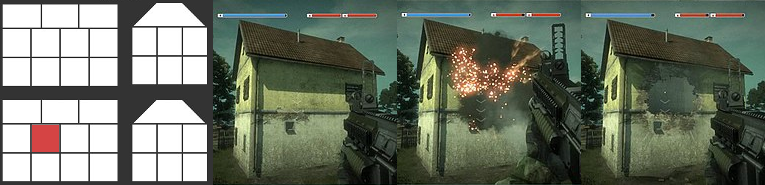
\includegraphics[width=\textwidth]{img/frostbite}
\caption{The arrangement of destructible elements for the large-scale destruction in \emph{Frostbite} engine (on the left). Rest of the images shows the process of large-scale destruction in \emph{Battlefield: Bad Company} implemented using \emph{Frostbite 1}.}
\label{fig:frostbite}
\end{figure}

\section{Methods and algorithms}

Here we will give a short overview of several more rigorous algorithms commonly used for simulations of destructible environment. 

In simulations, we consider two types of objects: soft bodies and rigid bodies. A rigid body represents an object with a constant shape. It means that every two points on the body are always in the same relative position. On the other hand, soft bodies are deformable under an applied force, meaning a point on the body can change its position independently on every other point. Although there are no actual rigid objects in the real world, soft body simulation is computationally more expensive than the rigid body. Therefore, in the computer games, rigid body simulation is used almost exclusively. This brings us to the problem of imitating the soft body behaviour on a rigid body in the real-time simulation. 

It is worth mentioning that many soft bodies in the games players can not directly interact with, \eg waving flag or flowing water, are implemented as a pre-rendered animations and not actual simulations. The simulation of those objects would not bring any value from a gameplay perspective, but it would require a lot of processing power that could be used elsewhere. 

\subsection{Soft body deformation}
In this section, we will shortly introduce two different approaches for simulation of soft bodies. Despite the fact that soft bodies are currently not used in computer games to the extent of destructible environment, a few soft body objects can show up in a game. We also expect that with an evolution of more powerful hardware, soft body deformation will make its way into the gaming world.
\label{sec:softBody}

\para{Finite Element Method} (FEM) is a numerical method used to simulate the behaviour of a system that can be modelled by solving the same problem for the smaller discrete parts, called finite elements. Each element calculates its physical state, \eg stress or temperature, and propagates the results to neighbouring elements. This model can be used for simulation of fluid dynamics, brittle fractures~\cite{brittlefracture}, ductility~\cite{ductilefracture}, elasticity, heat transfer and other physical properties. It is beneficial in engineering, modelling and rendering scenes for computer generated images ~\cite{Bargteil:2007:AFE}. 
FEM requires a lot of computational resources and is mostly used in simulations that are not in real-time constraints. The algorithms like \citet{femingames} propose, that optimised version of FEM can be used in computer games. 

\para{Material point method} (MPM) is used to simulate the behaviour of continuum materials, continuum material is represented as continuous mass not a set of discrete particles. MPM is a particle method and uses material points (Lagrangian elements) to describe a body. Each material point stores and calculates its position, velocity and deformation gradient. The difference between MPM and FEM is that the MPM is a meshfree method. Meshfree method stores all its information in the particles and avoids numerical errors from remeshing algorithms. In the context of numerical method MPM is an Arbitrary Lagrangian–Eulerian numerical method \cite{ALE}, this means that calculations do not only use material points, but also a Eulerian grid. A simplified overview of algorithm steps follows, for more details see the thesis of \citet{jiang2015material}.

\begin{enumerate}
    \item Grid data are reinitialized to default values.
    \item Weights and weight gradients are computed on every particle.
    \item Mass and momentum are transferred from the particles to the grid.
    \item The explicit forces on nodes are calculated
    \item The explicit nodal velocity update is performed
    \item Grid based collision is performed on vertices.
    \item Particles are updated from grid velocities.
\end{enumerate}
These steps are illustrated in \cref{fig:mpm}.

MPM is useful for both fluid and soft body dynamics. It can simulate deformation, fractures, heat transfer, melting and other changes of the state of an object.

A popular example of MPM deployment can be seen in snow simulation in the \emph{Disney} film \emph{Frozen (2013)}. The simulation software \emph{Matterhorn}\footnote{https://www.disneyanimation.com/technology/innovations/matterhorn} computes the behaviour of different types of snow (\eg wet, fresh, sticky) and other materials, such as sand or mud.

\begin{figure}
\centering
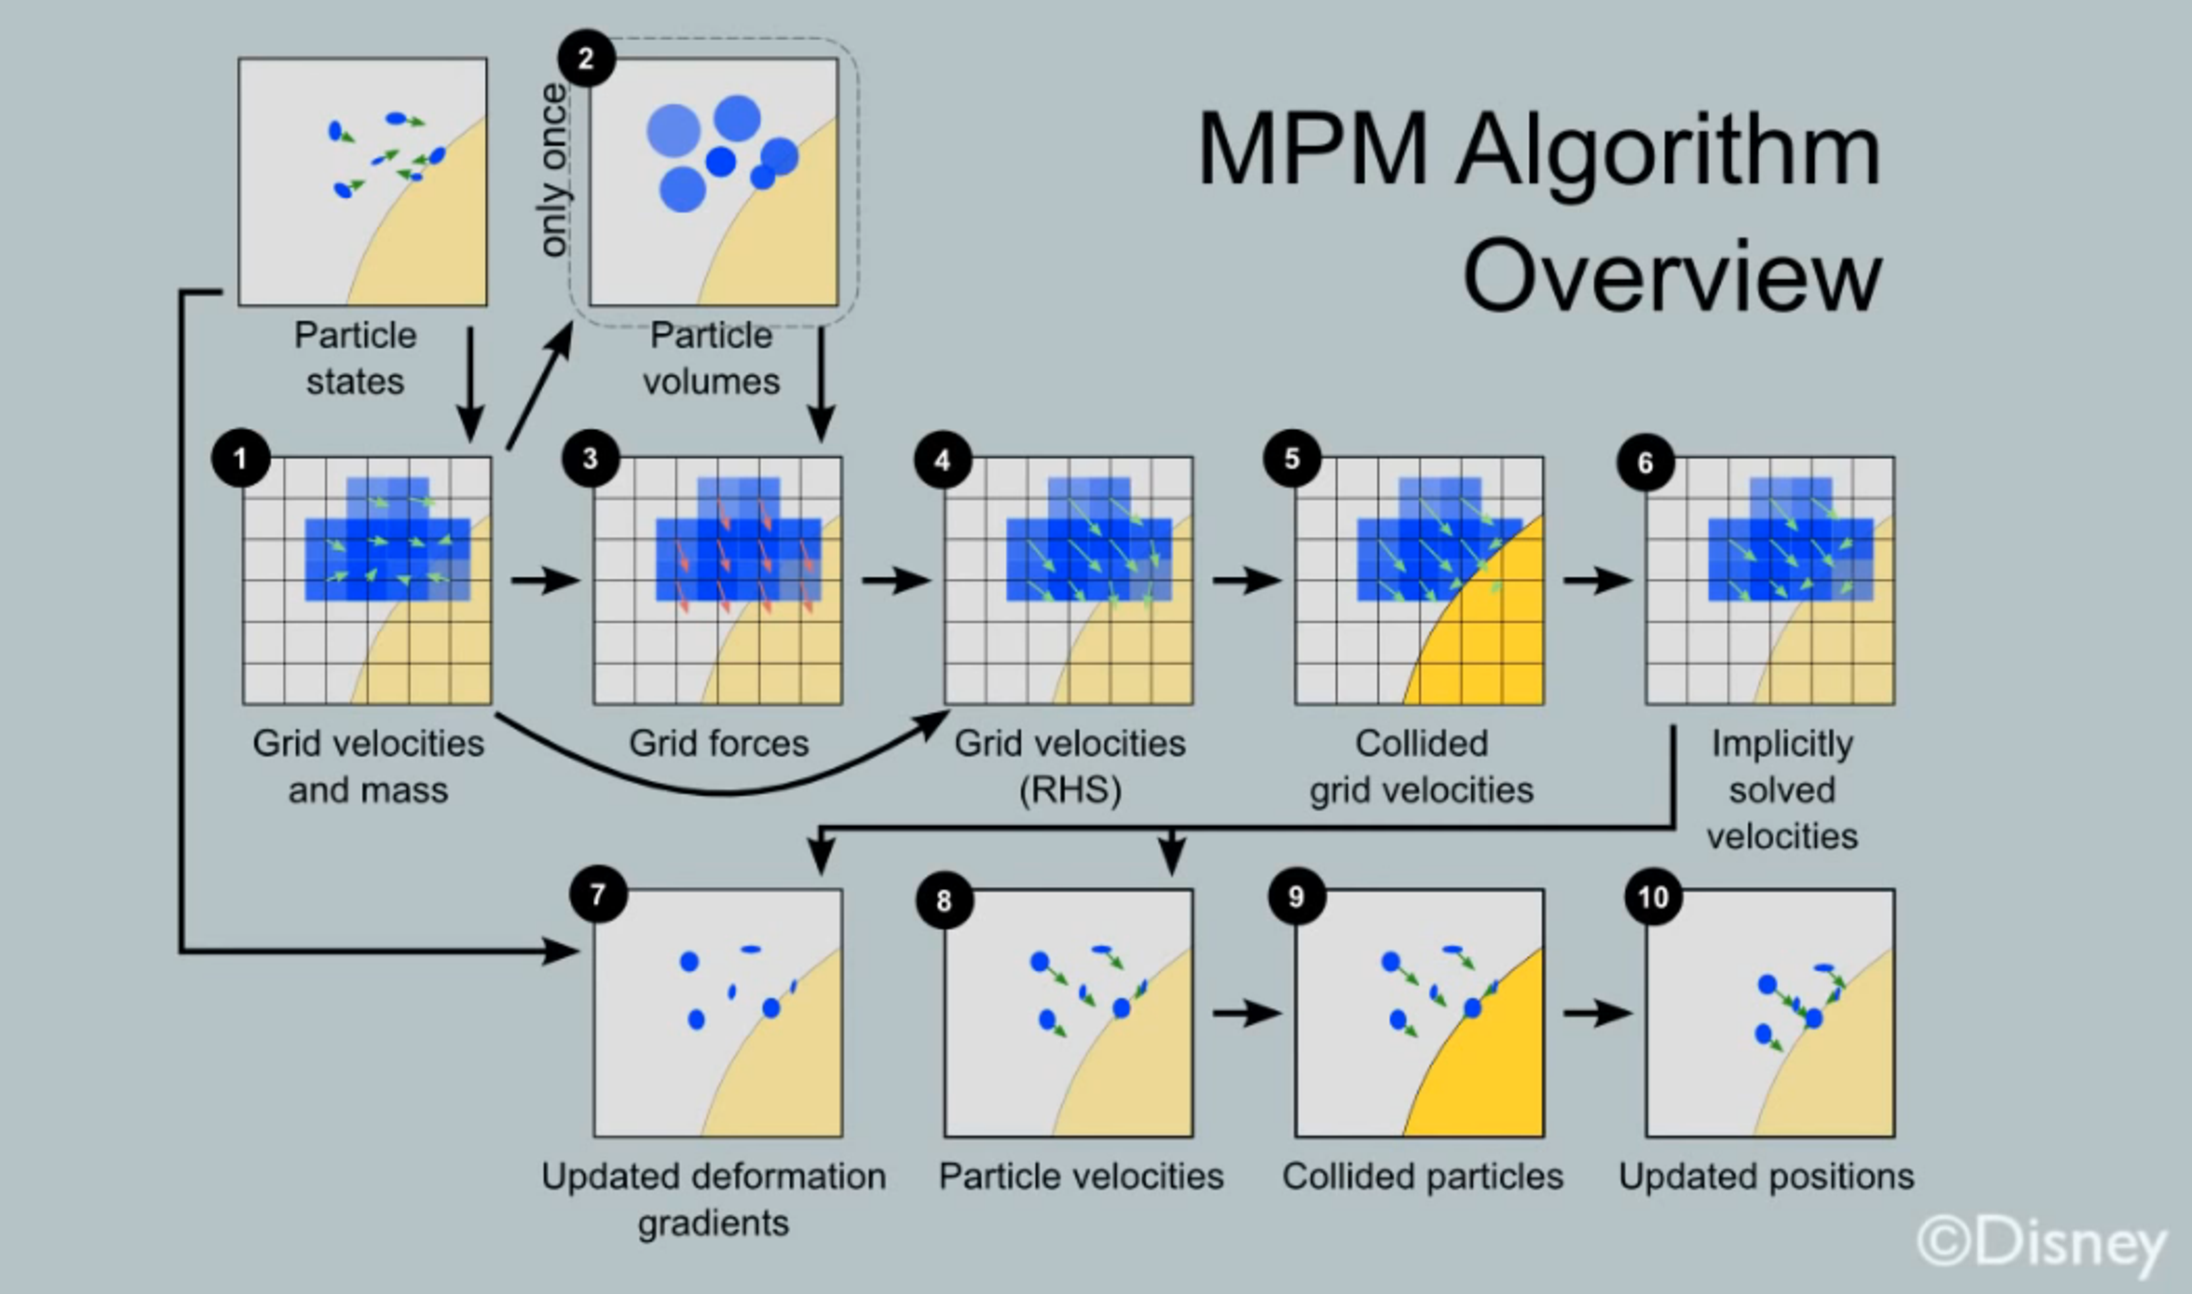
\includegraphics[width=\textwidth]{img/MPM}
\caption{Material point method algorithm overview. The top and the bottom rows operate in particle domain (Lagrangian) while the middle depicts grid-based (Eulerian) operations \cite{disney}.
}
\label{fig:mpm}
\end{figure}

\subsection{Rigid body decomposition}
In the soft body, application of the force propagates across the particles, and the connected particles break apart when the limit is exceeded. This creates the fracturing that may lead to the whole body splitting. In the rigid body simulation, the body has no internal structure, and therefore the applied force can only change the momentum of the entire body. This prohibits the deformation or fracturing a rigid body in a simulation.

To handle this problem, there are numerous approaches of decomposing the rigid body in the way that imitates fractures achieved by exceeding the elasticity of the material. The most common approach is a decomposition of a rigid body into smaller parts. A few of the methods for decomposition are slicing by planes, convex decomposition, tetrahedralization and Voronoi tessellation. 

\para{Voronoi tessellation} is a method of decomposing a solid object into smaller parts, as shown on \cref{fig:voro}. It is also applicable for \eg terrain generation~\cite{voronoiterrainrealtime}, but we will focus on object decomposition. Assuming the input is a closed triangular mesh with non-empty volume, the tessellation can be done in following three steps:

\begin{figure}
        \centering
        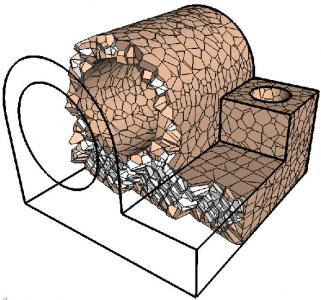
\includegraphics[width=0.4\textwidth]{img/clipped}
        \caption{The result of Voronoi tessellation \cite{yan2010efficient}}
        \label{fig:voro}
\end{figure}

\begin{description}
    \item[Delaunay tetrahedral decomposition] Given points $P$ in general position (the vertices of input mesh and a set of points inside its volume), tetrahedral mesh $DT(P)$ can be generated satisfying the following condition: no point in $P$ is inside the circumscribed sphere of any tetrahedra in $DT(P)$~\cite{cignoni1993parallel}.
    \item[Creating Voronoi diagram] For a Delaunay tetrahedral decomposition, its dual graph (with vertices in the centre of tetrahedrons circumscribed sphere) is a Voronoi diagram (see \cref{fig:voro}).
    
 \begin{figure}
    \centering
    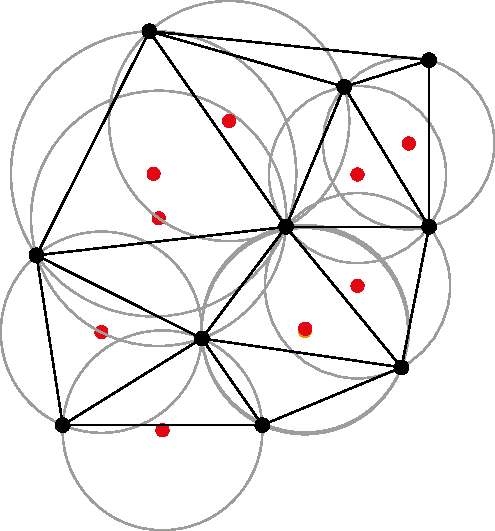
\includegraphics[width=0.4\textwidth]{img/delaunay}
    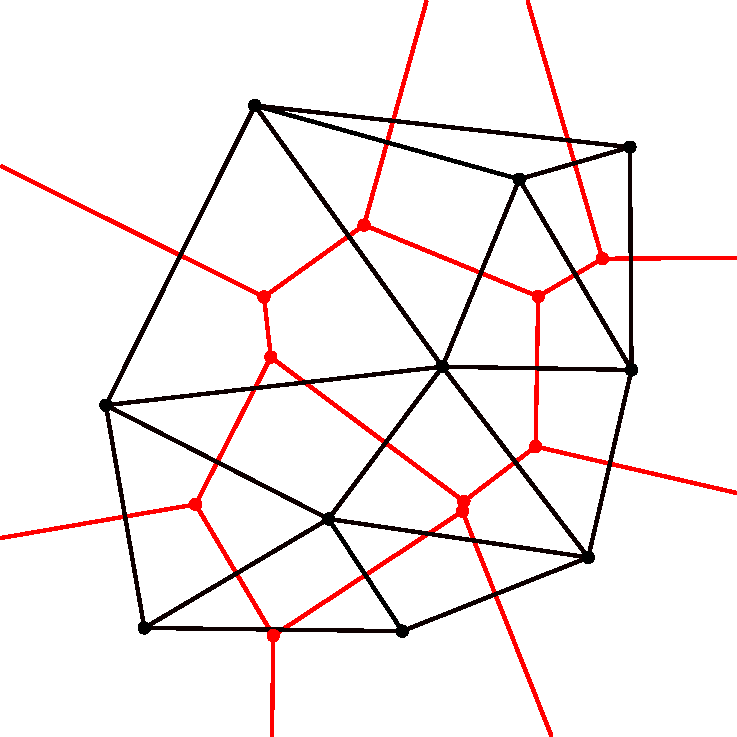
\includegraphics[width=0.4\textwidth]{img/voronoi}
    \caption{Transformation of 2D Delaunay triangulation to Voronoi diagram. Source: \url{https://en.wikipedia.org/wiki/Delaunay\_triangulation}}
    \label{fig:DT}
\end{figure}

    \item[Clipping the Voronoi diagram] Boundary cells of the Voronoi diagram are infinite (see \cref{fig:DT}) and need to be clipped by the original input triangular mesh. The efficient algorithm proposed by~\citet{yan2010efficient} for this task finds the intersection of the boundary Voronoi cell with the triangular mesh and continues with neighbourhood propagation to determine all intersections. 
\end{description}


\todo{co s tim? Jak je ten voronojuv tesselation rychlej, jaky sou vysledky? Nebylo by spatny dat \\ref na nejakou kapitolu kde to pouzijes}

\section{Related research}
In this section, we review two results of recent research which propose different techniques for environment destruction in computer games. First technique will focus on simulating the forces inside the object with the approach based on particle methods. The second one will solely focus on the destruction of rigid bodies with the use of Voronoi decomposition. 

\subsection{A fast method for simulating destruction and the generated dust
and debris}
\label{sec:edem}
The method of \citet{edem} approaches destruction on three scales. At first, the destruction is performed on a coarse scale, and then the applied energy is used to calculate the amount and size of smaller debris and finally dust particles.

\begin{description}
\item[Destruction on a coarse scale] on this level the authors use Extended Distinct Element Method (EDEM) which is based on Element Method described in section \ref{sec:softBody}. Instead of using particles, EDEM uses a set of rigid bodies that need to be produced by some tessellation method. The extension over traditional DEM is the use of pore springs connecting the adjacent elements. The authors compare the elements to individual bricks (the distinct elements) held together by layers of mortar (the pore springs). If the applied force is sufficient and elements move apart far enough, the fracture takes place. Pore springs also help the object retain its original shape after applied force.
\begin{figure}[ht!]
        \centering
        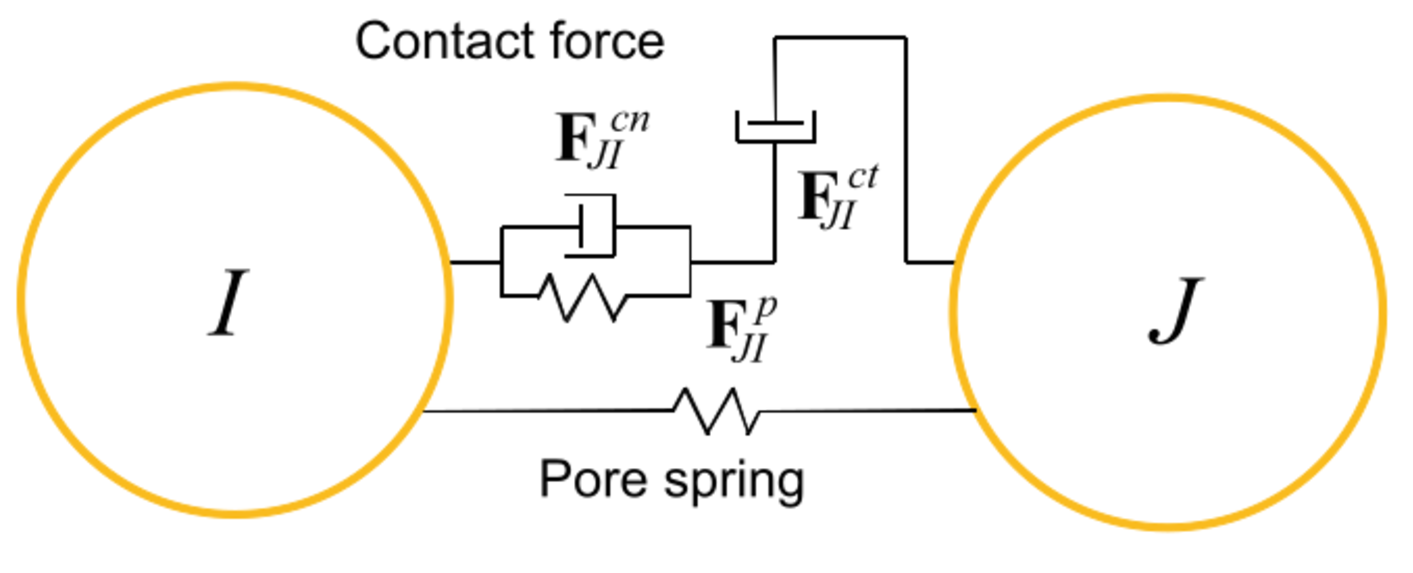
\includegraphics[width=0.7\textwidth]{img/spring}
        \caption{The force between two EDEM elements \cite{edem}}
        \label{spring}
\end{figure}
\\Algorithm for creating EDEM elements
\begin{enumerate}
\item Represent the original object as a closed surface model.
\item Arbitrarily arrange the EDEM elements inside the object.
Elements are allowed to overlap at this point.
\item Move elements by performing the EDEM simulation. Only the contact force will be considered in this simulation.
\item Perform collision detection between the object’s surface
and elements, making sure that they always
stay inside the object.
\item Repeat (3)–(4) until elements are stabilised.
\item Construct a Delaunay diagram from the set of elements
and put the pore springs on the Delaunay edges that connect
the elements
\end{enumerate}
The position $\mathbf{x}_I$ and velocity $\mathbf{v}_I$ of the element $\mathit{I}$ can be found using Newton’s equation of motion as follows:
 
\[M\frac{d\mathbf{v}_I}{dt} = \sum_{J \in contact}^{} \mathbf{F}_{JI}^c + \sum_{K \in pore}^{} \mathbf{F}_{KI}^p + M\mathbf{g} \]
\[ \frac{d\mathbf{x}_I}{dt} = \mathbf{v}_I \]
Here, $\mathbf{g}$ is the gravitational vector, $\mathbf{F}^c_{JI}$ is the contact force, $\mathbf{F}^p_{KI}$ is the force due to the pore springs and $\mathit{M}$ is the element’s mass. Two elements \{I, J\} are in contact, if they are closer to each other than the diameter of a single element.

\item[Fine debris generation and simulation] If a fracture between EDEM elements happened, we can determine if there was enough energy to break EDEM element into smaller debris. The probability distribution is used to determine the size of debris. Debris is taken out of EDEM simulation and put into particle simulation, where each piece is represented as a particle without volume.

\item[Dust generation and simulation] Amount of generated dust is based on fracture energy and results of debris generation. Instead of simulating particles smaller than predetermined margin, they are represented as dust in a grid-based fluid simulation. The density of particular cell represents the amount of dust.

\end{description}

 \begin{figure}
        \centering
        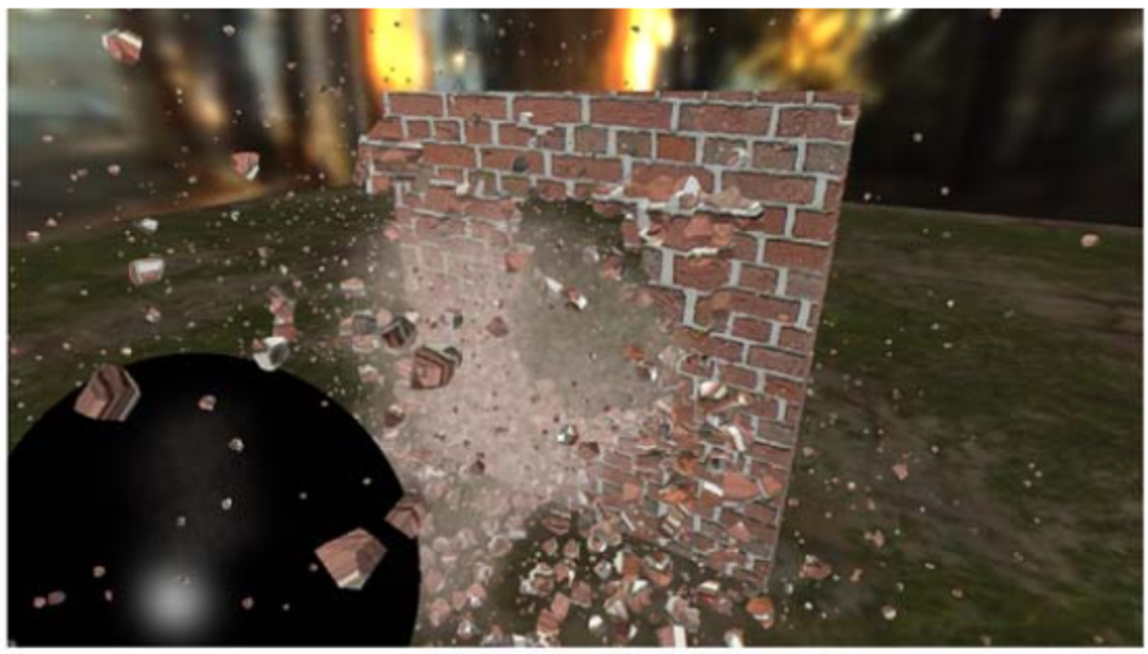
\includegraphics[width=0.49\textwidth]{img/edem_real}
        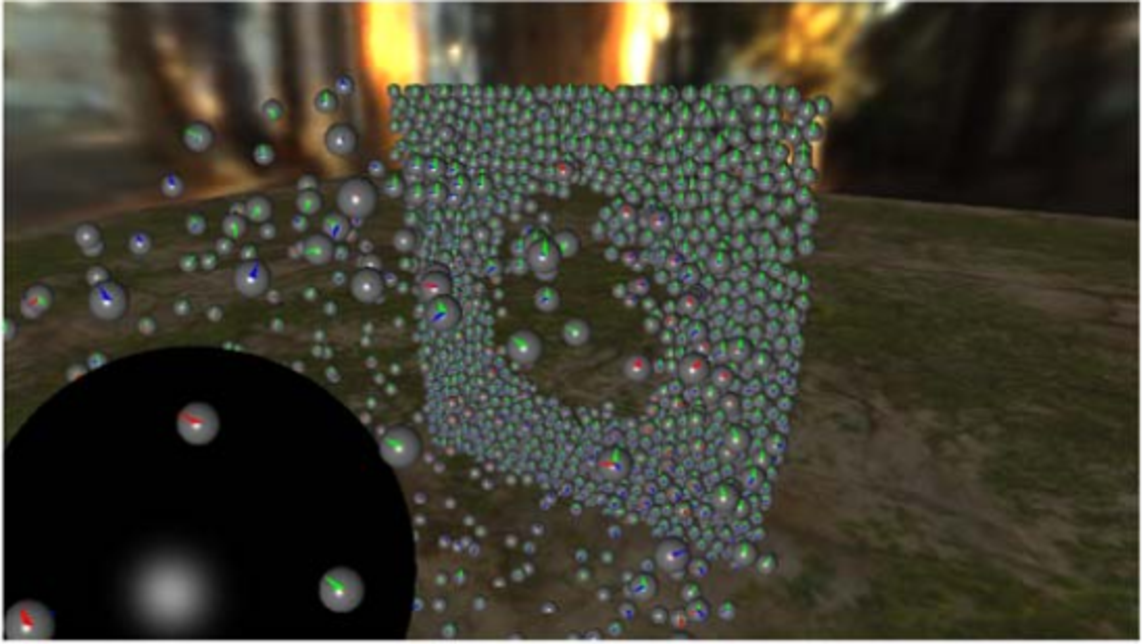
\includegraphics[width=0.49\textwidth]{img/edem}
        \caption{Result of this method with generated dust and debris (left) and EDEM elements (right) \cite{edem}}
        \label{fig:edem}
    \end{figure}
   
\begin{table}[ht!]
    \begin{center}
  \begin{tabular}{ |l|c|c|c|c|c| } 
  \hline
  EDEM elements & 128 & 256 & 512 & 1024 & 2048 \\ 
  \hline
  FPS & 320 & 160 & 75 & 30 & 9.1 \\ 
  \hline
  
  \end{tabular}
  \end{center}
  \caption{Performance of EDEM element method without rendering \cite{edem}}
  \label{table1}
\end{table}
In conclusion, based on table \ref{table1}, the frames per second (fps) drop proportionally with growing number of EDEM elements. The method achieved interactive fps on moderate number of EDEM elements. In addition the proposed debris and dust generation can be combined with other methods.

\subsection{Real Time Dynamic Fracture
with Volumetric Approximate Convex Decompositions}
\label{sec:RTDF}
The approach of \citet{nvidia} does not try to simulate the internal forces of an object and focuses only on rigid body decomposition. The idea behind this method is to represent the mesh as a compound shape of convex parts. The algorithm used for convex decomposition is Volumetric Approximate Convex Decomposition (VACD), which works by introducing the Voronoi decomposition into the bounding box of a mesh and then clipping the Voronoi cells by the mesh. The fracture pattern is precomputed and represented as a set of convex cells. The algorithm works as follows (\cref{fig:vacdalg}:
\begin{enumerate}
\item The fracture pattern is aligned with the point of impact, and rotated and scaled randomly to avoid an occurrence of same-looking patterns.
\item The intersections of all cells with all convex parts are computed. To compute the intersection of a single cell with a single convex part, the convex part is clipped against all the planes of the cell one by one. 
At the end of this step, we have a set of new convex parts, and each convex part belongs to exactly one cell.
\item If there are convex parts that together entirely fill one cell, we can combine them into single new one convex part. The test is carried out using a simple volume comparison.
\item All convex parts that belong to one cell are combined to form a new compound part. This ensures that the temporary parts of decomposition into compound shape are not visible after the fracture (see \cref{fig:vacdfracture}).
\begin{figure}
        \centering
        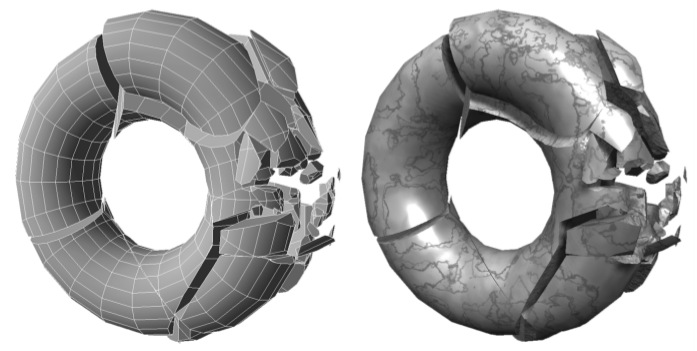
\includegraphics[width=0.7\textwidth]{img/vacdfracture}
        \caption{The decomposition to the
initial compound mesh does not become visible when a fracture
pattern is applied. Source: \citet{nvidia}}
        \label{fig:vacdfracture}
\end{figure}
\item Finally, the separate islands of convex parts are detected and individual compound shapes are constructed for them.
\end{enumerate}

\begin{figure}
\centering
        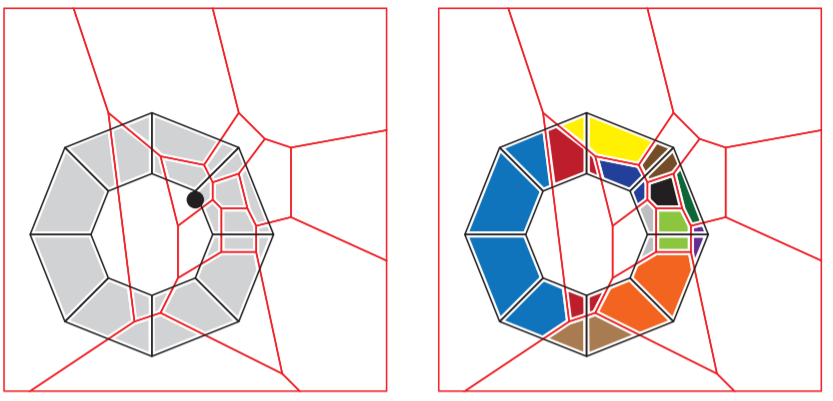
\includegraphics[width=\textwidth]{img/vacdAlgorithm}
        \caption{Overview of the fracture algorithm. Left: The fracture pattern (red) is aligned with the impact location (black dot). Middle: All
convex pieces are intersected with all cells. The green convex pieces can be welded to form a single piece because they cover the entire
cell. Pieces within one cell become a new compound (colouring). Island detection finds that the dark red compound needs to be split. Source: \citet{nvidia}}
        \label{fig:vacdalg}
\end{figure}

The cost of fracturing in this method depends only on the number of mesh triangles of the object being fractured and the resolution of fracture pattern. The paper suggests that the model with $10^6$ vertices and $5\cdot10^5$ faces can be fractured under 50ms. This makes this method suitable for real-time computer games.

